% !TEX program = xelatex
% Example: Animated TikZ diagram in Beamer
% Uses \onslide<1->, <2->, <3-> to reveal a flowchart step by step.
\documentclass{beamer}
\usetheme{default}
\usepackage{tikz}
\usetikzlibrary{positioning, arrows.meta, shapes.geometric}

\title{Animated TikZ in Beamer}
\author{Dr.~Edsger Dijkstra}
\institute{University of Texas}
\date{2025}

\begin{document}

\begin{frame}
  \titlepage
\end{frame}

\begin{frame}{A Step-by-Step Flowchart}
  \begin{center}
    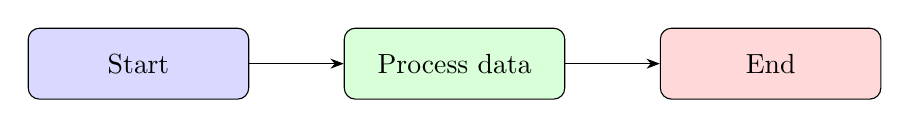
\begin{tikzpicture}[node distance=1.2cm,
        every node/.style={draw, rounded corners,
          minimum width=2.8cm, minimum height=0.9cm, align=center}]
      \onslide<1->{\node[fill=blue!15] (start) {Start};}
      \onslide<2->{\node[fill=green!15, right=of start] (proc) {Process data};}
      \onslide<3->{\node[fill=red!15, right=of proc] (end) {End};}
      \onslide<2->{\draw[-Stealth] (start) -- (proc);}
      \onslide<3->{\draw[-Stealth] (proc) -- (end);}
    \end{tikzpicture}
  \end{center}
  \vspace{0.5em}
  \begin{itemize}
    \item<1-> The start node appears first.
    \item<2-> The process node and arrow appear next.
    \item<3-> The end node completes the diagram.
  \end{itemize}
\end{frame}

\end{document}
